\documentclass[11pt]{article}
\pagestyle{plain}

% \pgfplotsset{compat=1.18}
\usepackage[margin=1in]{geometry}
\usepackage{amsmath,amsfonts,amssymb,amsthm}
\usepackage[ruled,vlined,linesnumbered,commentsnumbered]{algorithm2e}
\SetKwInput{KwIn}{Input}
\SetKwInput{KwOut}{Output}
\SetKwInput{KwGlobal}{Global variable}
\SetKwInput{KwOracle}{Oracle}
\SetKwComment{Comment}{// }{}
\usepackage{graphicx}
\usepackage{enumerate}
\usepackage{bbm}
\usepackage{verbatim}
\usepackage{hyperref,color}
\usepackage[capitalize,nameinlink]{cleveref}
\usepackage[dvipsnames]{xcolor}
\hypersetup{
	colorlinks=true,
	pdfpagemode=UseNone,
	citecolor=OliveGreen,
	linkcolor=NavyBlue,
	urlcolor=Magenta,
	pdfstartview=FitW
}
\usepackage{appendix}
\usepackage{makecell}
\usepackage{tablefootnote}
\crefname{appsec}{Appendix}{Appendices}
\usepackage{tikz}
\usetikzlibrary{arrows.meta,calc}
\usepackage{pgfplots}
\usepackage{xifthen}
\usepackage{subcaption}
\usepackage{hhline}

\theoremstyle{plain}
\newtheorem{theorem}{Theorem}[section]
\newtheorem{proposition}[theorem]{Proposition}
\newtheorem{lemma}[theorem]{Lemma}
\newtheorem{corollary}[theorem]{Corollary}
\newtheorem{conjecture}[theorem]{Conjecture}
\newtheorem{problem}[theorem]{Problem}
\newtheorem{claim}[theorem]{Claim}
\newtheorem{fact}[theorem]{Fact}

\theoremstyle{definition}
\newtheorem{definition}[theorem]{Definition}
\newtheorem{example}[theorem]{Example}
\newtheorem{observation}[theorem]{Observation}
\newtheorem{assumption}[theorem]{Assumption}
\newtheorem*{assumption*}{Assumption}
\newtheorem{condition}[theorem]{Condition}

\theoremstyle{remark}
\newtheorem{remark}[theorem]{Remark}

\crefname{lemma}{Lemma}{Lemmas}
\crefname{theorem}{Theorem}{Theorems}
\crefname{definition}{Definition}{Definitions}
\crefname{fact}{Fact}{Facts}
\crefname{claim}{Claim}{Claims}
\crefname{proposition}{Proposition}{Propositions}


\newcommand{\dif}{\,\mathrm{d}}
%\newcommand{\E}{\mathbb{E}}
%\newcommand{\Var}{\mathrm{Var}}
\newcommand{\Cov}{\mathrm{Cov}}
\newcommand{\MI}{\mathrm{I}}
%\newcommand{\Ent}{\mathrm{Ent}}
\newcommand{\ind}{\mathbbm{1}}
\newcommand{\allone}{\mathbf{1}}
\newcommand{\tr}{\mathrm{tr}}
\newcommand{\wt}{\mathrm{weight}}
\DeclareMathOperator*{\argmax}{arg\,max}
\newcommand{\norm}[1]{\left\lVert #1 \right\rVert}
\newcommand{\TV}[2]{\left\|#1 - #2\right\|_{\mathrm{TV}}}
\newcommand{\ceil}[1]{\left\lceil #1 \right\rceil}
\newcommand{\floor}[1]{\left\lfloor #1 \right\rfloor}
\newcommand{\ip}[2]{\left\langle #1 , #2 \right\rangle}
\newcommand{\grad}{\nabla}
\newcommand{\hessian}{\nabla^2}
\newcommand{\trans}{\intercal}
\newcommand{\diag}{\mathrm{diag}}
\newcommand{\poly}{\mathrm{poly}}
\newcommand{\dist}{\mathrm{dist}}
\newcommand{\sgn}{\mathrm{sgn}}
\newcommand{\fpras}{\mathsf{FPRAS}}
\newcommand{\fpaus}{\mathsf{FPAUS}}
\newcommand{\fptas}{\mathsf{FPTAS}}

\newcommand{\eps}{\varepsilon}

\newcommand{\N}{\mathbb{N}}
\newcommand{\Z}{\mathbb{Z}}
\newcommand{\Q}{\mathbb{Q}}
\newcommand{\R}{\mathbb{R}}
\newcommand{\C}{\mathbb{C}}

\renewcommand{\AA}{\mathcal{A}}
\newcommand{\BB}{\mathcal{B}}
\newcommand{\CC}{\mathcal{C}}
\newcommand{\DD}{\mathcal{D}}
\newcommand{\EE}{\mathcal{E}}
\newcommand{\FF}{\mathcal{F}}
\newcommand{\GG}{\mathcal{G}}
\newcommand{\HH}{\mathcal{H}}
\newcommand{\II}{\mathcal{I}}
\newcommand{\JJ}{\mathcal{J}}
\newcommand{\KK}{\mathcal{K}}
\newcommand{\LL}{\mathcal{L}}
\newcommand{\MM}{\mathcal{M}}
\newcommand{\NN}{\mathcal{N}}
\newcommand{\OO}{\mathcal{O}}
\newcommand{\PP}{\mathcal{P}}
\newcommand{\QQ}{\mathcal{Q}}
\newcommand{\RR}{\mathcal{R}}
\renewcommand{\SS}{\mathcal{S}}
\newcommand{\TT}{\mathcal{T}}
\newcommand{\UU}{\mathcal{U}}
\newcommand{\VV}{\mathcal{V}}
\newcommand{\WW}{\mathcal{W}}
\newcommand{\XX}{\mathcal{X}}
\newcommand{\YY}{\mathcal{Y}}
\newcommand{\ZZ}{\mathcal{Z}}

\newcommand{\KL}[2]{D_{\mathrm{KL}} \left( #1 \,\Vert\, #2 \right)}
\newcommand{\KLbig}[2]{D_{\mathrm{KL}} \left( #1 \,\big\Vert\, #2 \right)}
\newcommand{\KLBig}[2]{D_{\mathrm{KL}} \left( #1 \,\Big\Vert\, #2 \right)}

\newcommand{\SKL}[2]{D_{\mathrm{SKL}} \left( #1 \,\Vert\, #2 \right)}
\newcommand{\SKLbig}[2]{D_{\mathrm{SKL}} \left( #1 \,\big\Vert\, #2 \right)}
\newcommand{\SKLBig}[2]{D_{\mathrm{SKL}} \left( #1 \,\Big\Vert\, #2 \right)}

\newcommand{\qandq}{\quad\text{and}\quad}
\newcommand{\supp}{\mathrm{supp}}

\newcommand{\DKL}[2]{\-D_{\-{KL}}\left(#1 \parallel #2\right)}
\newcommand{\DTV}[2]{\-D_{\mathrm{TV}}\left({#1},{#2}\right)}
% \newcommand{\dist}{\mathrm{dist}}
\newcommand{\e}{\mathrm{e}}
\renewcommand{\epsilon}{\varepsilon}
\renewcommand{\emptyset}{\varnothing}
% \newcommand{\norm}[1]{\left\Vert#1\right\Vert}
\newcommand{\set}[1]{\left\{#1\right\}}
\newcommand{\tuple}[1]{\left(#1\right)} 
% \newcommand{\eps}{\varepsilon}
\newcommand{\inner}[2]{\left\langle #1,#2\right\rangle}
\newcommand{\tp}{\tuple}
\newcommand{\ol}{\overline}
\newcommand{\abs}[1]{\left\vert#1\right\vert}
\newcommand{\ctp}[1]{\left\lceil#1\right\rceil}
\newcommand{\ftp}[1]{\left\lfloor#1\right\rfloor}
\newcommand{\Ind}[1]{\-{Ind}_{#1}}
\newcommand{\todo}[1]{{\color{red} TODO: #1}}

\newcommand{\Cor}{\Psi^{\mathrm{sym}}}
\newcommand{\cor}{\Psi^{\-{cor}}}
\newcommand{\Inf}{\Psi}
% \newcommand{\diag}{\-{diag}}

\def\*#1{\boldsymbol{#1}} % Use \*A for \mathbf{A}
\def\+#1{\mathcal{#1}} % Use \+A for \mathcal{A}
\def\-#1{\mathrm{#1}} % Use \-A for \mathrm{A}
\def\=#1{\mathbb{#1}} % Use \^A for \mathbb{A}
\def\!#1{\mathfrak{#1}} % Use \!A for \mathfrak{A}

\newcommand*\diff{\mathop{}\!\mathrm{d}}

% probability
% \DeclareMathOperator*{\oPr}{\mathbf{Pr}}
\def\oPr{\mathop{\mathrm{Pr}}}
\renewcommand{\Pr}[2][]{ \ifthenelse{\isempty{#1}}
  {\oPr\left[#2\right]}
  {\oPr_{#1}\left[#2\right]} } % Use \Pr[a]{b} for \mathbf{Pr}_a[b], \Pr{b} for  \mathbf{Pr}[b]

% expectation: relies on the package "dsfont"
% \DeclareMathOperator*{\oE}{\mathbb{E}}
\def\oE{\mathop{\mathbb{E}}}
\newcommand{\E}[2][]{ \ifthenelse{\isempty{#1}}
  {\oE\left[#2\right]}
  {\oE_{#1}\left[#2\right]} }

% variance
%\DeclareMathOperator*{\oVar}{\mathbf{Var}}
\def\oVar{\mathrm{Var}}
\newcommand{\Var}[2][]{ \ifthenelse{\isempty{#1}}
  {\oVar\left[#2\right]}
  {\oVar_{#1}\left[#2\right]} }

% entropy
% \DeclareMathOperator*{\oEnt}{\mathbf{Ent}}
\def\oEnt{\mathrm{Ent}}
\newcommand{\Ent}[2][]{ \ifthenelse{\isempty{#1}}
  {\oEnt\left[#2\right]}
  {\oEnt_{#1}\left[#2\right]} }

\newcommand{\PhiEnt}[2][]{ \ifthenelse{\isempty{#1}}
  {\oEnt^\phi\left[#2\right]}
  {\oEnt^\phi_{#1}\left[#2\right]} }


\newenvironment{Exampleparagraph}[1][]
{
    \par 
    \noindent 
    \textbf{\color{blue} #1}
    \par 
    \vspace{0.5em} 
    \itshape 
}
{
    \par 
    \vspace{1em} 
}

%\input{local-macro}

\newcommand{\RED}[1]{\textcolor{red}{#1}}
\newcommand{\zc}[1]{\textcolor{red}{ZC: #1}}

\newcommand{\bern}[1]{\mathrm{Bern}\left(#1\right)}



\title{Note on Reinforced Bakry-Emery Condition}
\date{\today}

\pgfplotsset{compat=1.18} 
\begin{document}

\maketitle

\section{RBE to local Bobkov}
\paragraph{Setup}
Let $\mu$ be a distribution over $\{-1,+1\}^n$ and $Lf(x) = \sum_{i=1}^n p_i(x) (f(x^{\oplus i}) - f(x))$ be the infinisimal generator of a Markov chain reversible w.r.t. $\mu$.
Let $P_t = \e^{tL}$ be the continuous-time Markov semigroup generated by $L$.
Let $I(r)=\varphi(\Phi^{-1}(r))$ be the Gaussian isoperimetric profile.
Define 
\begin{align*}
    \Gamma(f,g) &= \frac{1}{2} \tp{L(fg) - f Lg - g Lf} \\
    \Gamma_2(f,g) &= \frac{1}{2} (L\Gamma(f,g) - \Gamma(f, Lg) - \Gamma(Lf, g))
\end{align*}

\begin{fact}[Basic calculations]
For any $f,g:\{-1,+1\}^n \to \R$ and $x\in\{-1,+1\}^n$, we have
\begin{align*}
    \Gamma(f,g)(x) = \frac{1}{2} \sum_{i=1}^n p_i(x) (f(x^{\oplus i}) - f(x)) (g(x^{\oplus i}) - g(x)).
\end{align*}
Let $f_t = P_t f$. It holds
\begin{align*}
    \frac{\dif}{\dif t} \Gamma(f_t) = 2\Gamma(f_t,Lf_t),
    \qquad
    (L-\partial_t)\Gamma(f_t)=2\Gamma_2(f_t).
\end{align*}
Finally, it holds
\begin{align*}
    \Gamma(\sqrt{f^2 + g^2}) \le \Gamma(f) + \Gamma(g).
\end{align*}
\end{fact}

\begin{definition}[Reinforced Bakry-Emery condition]
We say the Markov chain satisfies $\mathrm{RBE}(\rho)$ if for any $f:\{-1,+1\}^n \to \R$ and $x\in\{-1,+1\}^n$, we have
\begin{align*}
    \Gamma(\sqrt{\Gamma(f)})(x) \le \Gamma_2(f)(x) - \rho \cdot \Gamma(f)(x).
\end{align*}
\end{definition}

\begin{theorem}
    Suppose the Markov chain satisfies $\mathrm{RBE}(\rho)$ for some $\rho>0$.
    Then for any $t\ge0$ and $f:\{-1,+1\}^n\to[0,1]$, the following local Bobkov inequality holds:
    \begin{align*}
        I\tp{P_t f}
        \le
        P_t \tp{\sqrt{I(f)^2 + \frac{2(1-\e^{-2\rho t})}{\rho} \cdot \Gamma(f)}}.
    \end{align*}
\end{theorem}

\begin{proof}
    Let $u_s=f_{t-s}=P_{t-s}f$ and
    \begin{align*}
        \gamma(s)=\frac{2(1-\e^{-2\rho s})}{\rho}.
    \end{align*}
    Define
    \begin{align*}
        F_s = \sqrt{I(u_s)^2 + \gamma(s) \cdot \Gamma(u_s)}.
    \end{align*}
    Since $F_0=I(P_t f)$ and
    $F_t=\sqrt{I(f)^2+\gamma(t)\Gamma(f)}$, it suffices to show that
    \begin{align*}
       \forall x \in \{-1,+1\}^n,\quad \frac{\dif}{\dif s}(P_s F_s)(x) = P_s((L+\partial_s) F_s) \ge 0
    \end{align*}
    for every $s\in[0,t]$. We prove the stronger pointwise statement
    $(L+\partial_s)F_s\ge0$.

    Put
    \begin{align*}
        q_s=F_s^2=I(u_s)^2+\gamma(s)\Gamma(u_s).
    \end{align*}
    At points where $F_s>0$, the carré-du-champ identity gives
    \begin{align*}
        L F_s
        =
        \frac{Lq_s}{2F_s}-\frac{\Gamma(F_s)}{F_s},
        \qquad
        \partial_s F_s=\frac{\partial_s q_s}{2F_s}.
    \end{align*}
    Thus
    \begin{align}\label{eq:LF-reduction}
        (L+\partial_s)F_s
        =
        \frac{(L+\partial_s)q_s-2\Gamma(F_s)}{2F_s}.
    \end{align}
    If $F_s=0$, the same conclusion follows by replacing $q_s$ by
    $q_s+\varepsilon$ and letting $\varepsilon\downarrow0$.

    We now lower bound the numerator in \eqref{eq:LF-reduction}. Note that
    \begin{align}\label{eq:lip-bound}
        \Gamma(F_s)
        \le
        \Gamma(I(u_s))+\gamma(s)\Gamma(\sqrt{\Gamma(u_s)}).
    \end{align}
    Second, since $\partial_s u_s=-Lu_s$,
    \begin{align}\label{eq:gamma-evolution}
        (L+\partial_s)\Gamma(u_s)
        =
        L\Gamma(u_s)-2\Gamma(u_s,Lu_s)
        =
        2\Gamma_2(u_s).
    \end{align}
    Finally, the Gaussian isoperimetric profile satisfies the standard estimate
    \begin{align}\label{eq:I-profile}
        I(a)\tp{I(b)-I(a)-I'(a)(b-a)}\ge -(b-a)^2
        \qquad \text{for all }a,b\in[0,1].
    \end{align}
    Hence
    \begin{align}\label{eq:I-part}
        &(L+\partial_s)I(u_s)^2-2\Gamma(I(u_s)) \notag\\
        &\qquad =
        2I(u_s)\tp{LI(u_s)-I'(u_s)Lu_s} \notag\\
        &\qquad =
        2I(u_s)\sum_{i=1}^n p_i(x)
        \tp{I(u_s(x^{\oplus i}))-I(u_s(x))-I'(u_s(x))(u_s(x^{\oplus i})-u_s(x))} \notag\\
        &\qquad \ge
        -2\sum_{i=1}^n p_i(x)(u_s(x^{\oplus i})-u_s(x))^2
        =
        -4\Gamma(u_s).
    \end{align}
    Combining \eqref{eq:lip-bound}, \eqref{eq:gamma-evolution}, and
    \eqref{eq:I-part}, we obtain
    \begin{align*}
        (L+\partial_s)q_s-2\Gamma(F_s)
        &\ge
        \tp{\gamma'(s)-4}\Gamma(u_s)
        +2\gamma(s)\tp{\Gamma_2(u_s)-\Gamma(\sqrt{\Gamma(u_s)})}\\
        &\ge
        \tp{\gamma'(s)-4+2\rho\gamma(s)}\Gamma(u_s).
    \end{align*}
    The last step uses $\mathrm{RBE}(\rho)$. Our choice of $\gamma$ satisfies
    $\gamma'(s)=4-2\rho\gamma(s)$, so the right-hand side is zero. Therefore
    $(L+\partial_s)F_s\ge0$, and the desired inequality follows by integrating
    the monotonicity of $P_sF_s$ from $s=0$ to $s=t$.
\end{proof}

\begin{corollary}[Bobkov inequality]
    If the Markov chain satisfies $\mathrm{RBE}(\rho)$ for some $\rho>0$, then for any $f:\{-1,+1\}^n\to[0,1]$, it holds
    \begin{align*}
        I\tp{\E{f}} \le \E{\sqrt{I(f)^2 + \frac{2}{\rho} \cdot \Gamma(f)}}.
    \end{align*}
\end{corollary}

\section{(reinforced) Bekry-Emery condition, (local) Bobkov inequalities and functional inequalities}

As shown in section 1, reinforced Bakry-Emery condition implies local Bobkov inequality, which again implies the Bobkov inequality.
Here, we show that Bobkov inequality can imply the following modified log-Sobolev inequality of the gradient type:
\begin{proposition}
    Bobkov inequality with parameter $\rho > 0$ implies the modified log-Sobolev inequality of the gradient type, i.e., for any $f: \{-1,+1\}^n \to \mathbb{R}_{>0}$, we have
    \begin{align*}
        \Ent[\mu]{f} \le \frac{1}{\rho} \cdot \E[\mu]{\frac{\Gamma(f)}{f}}.
    \end{align*}
\end{proposition}
\begin{proof}
    Let $m=\E[\mu]{f}$. Since the state space is finite and $f>0$, we may
    choose $\epsilon>0$ so small that $\epsilon f\le 1$. Applying the Bobkov
    inequality to $\epsilon f$ gives
    \begin{align}\label{eq:bobkov-eps-f}
        \frac{I(\epsilon m)}{\epsilon}
        \le
        \E[\mu]{\sqrt{\tp{\frac{I(\epsilon f)}{\epsilon}}^2
        +\frac{2}{\rho}\Gamma(f)}} .
    \end{align}
    We use the following standard consequence of Mills' ratio: for every fixed
    finite set $A\subset(0,\infty)$, as $\epsilon\downarrow0$,
    \begin{align}\label{eq:I-small-expansion}
        \frac{I(\epsilon a)}{\epsilon}
        =
        a A_\epsilon
        +
        \frac{a\log(1/a)}{\sqrt{2\log(1/\epsilon)}}
        +
        o\left(\frac{1}{\sqrt{\log(1/\epsilon)}}\right)
        \qquad(a\in A),
    \end{align}
    uniformly in $a$, where $A_\epsilon$ is independent of $a$.
    Taking $A=\set{f(x):x\in\{-1,+1\}^n}\cup\set{m}$ in
    \eqref{eq:I-small-expansion}, the common leading term cancels and
    \begin{align}\label{eq:left-limit}
        \lim_{\epsilon\downarrow0}
        \sqrt{2\log(1/\epsilon)}
        \tp{
        \frac{I(\epsilon m)}{\epsilon}
        -
        \E[\mu]{\frac{I(\epsilon f)}{\epsilon}}
        }
        &=
        m\log(1/m)-\E[\mu]{f\log(1/f)} \notag\\
        &=
        \Ent[\mu]{f}.
    \end{align}
    On the other hand, since $I(\epsilon f)/\epsilon\sim
    f\sqrt{2\log(1/\epsilon)}$ pointwise,
    \begin{align}\label{eq:right-limit}
        &\lim_{\epsilon\downarrow0}
        \sqrt{2\log(1/\epsilon)}
        \E[\mu]{
        \sqrt{\tp{\frac{I(\epsilon f)}{\epsilon}}^2
        +\frac{2}{\rho}\Gamma(f)}
        -
        \frac{I(\epsilon f)}{\epsilon}
        } \notag\\
        &\qquad =
        \E[\mu]{
        \lim_{\epsilon\downarrow0}
        \frac{\sqrt{2\log(1/\epsilon)}\cdot \frac{2}{\rho}\Gamma(f)}
        {
        \sqrt{\tp{\frac{I(\epsilon f)}{\epsilon}}^2+\frac{2}{\rho}\Gamma(f)}
        +\frac{I(\epsilon f)}{\epsilon}
        }}
        =
        \frac{1}{\rho}\E[\mu]{\frac{\Gamma(f)}{f}} .
    \end{align}
    Subtracting $\E[\mu]{I(\epsilon f)/\epsilon}$ from both sides of
    \eqref{eq:bobkov-eps-f}, multiplying by $\sqrt{2\log(1/\epsilon)}$, and
    letting $\epsilon\downarrow0$, \eqref{eq:left-limit} and
    \eqref{eq:right-limit} yield
    \begin{align*}
        \Ent[\mu]{f}
        \le
        \frac{1}{\rho}\E[\mu]{\frac{\Gamma(f)}{f}}.
    \end{align*}
\end{proof}

\begin{remark}
    This type of modified log-Sobolev inequality is weaker than the standard one. See \url{https://tetali.math.gatech.edu/PUBLIS/BT_ENT.pdf}.
\end{remark}

\begin{remark}[$\mathrm{BE}$ does not imply $\mathrm{rBE}$]
    There is no universal constant loss from $\mathrm{BE}$ to $\mathrm{rBE}$:
    $\mathrm{BE}(\rho)$ does not imply $\mathrm{rBE}(\rho/C)$ for any
    $C>1$. This fails already for a weighted path chain on three sites. Let
    the state space be $\{0,1,2\}$ and let
    \begin{align*}
        Lf(0)=f(1)-f(0),\qquad
        Lf(1)=f(0)-f(1)+\frac{1}{2}(f(2)-f(1)),\qquad
        Lf(2)=\frac{1}{2}(f(1)-f(2)).
    \end{align*}
    Writing $d=f(0)-f(1)$ and $e=f(2)-f(1)$, one checks
    \begin{align*}
        \Gamma(f)(0)&=\frac{d^2}{2},
        &
        \Gamma_2(f)(0)&=\frac{7}{8}d^2+\frac{1}{8}(d+e)^2
        \ge \frac{7}{4}\Gamma(f)(0),\\
        \Gamma(f)(1)&=\frac{d^2}{2}+\frac{e^2}{4},
        &
        \Gamma_2(f)(1)&=\frac{7}{8}d^2+\frac{1}{2}de+\frac{1}{8}e^2
        \ge \frac{9-\sqrt{57}}{8}\Gamma(f)(1),\\
        \Gamma(f)(2)&=\frac{e^2}{4},
        &
        \Gamma_2(f)(2)&=\frac{1}{8}(d+e)^2+\frac{1}{8}e^2
        \ge \frac{1}{2}\Gamma(f)(2),
    \end{align*}
    where the middle-site constant is the smallest generalized eigenvalue of
    the displayed quadratic forms. Thus the chain satisfies $\mathrm{BE}(\rho)$
    for $\rho=(9-\sqrt{57})/8>0$. On the other hand, for $f_t=(-1,0,t)$, at the
    site $2$,
    \begin{align*}
        \Gamma(f_t)(2)&=\frac{t^2}{4},
        &
        \Gamma_2(f_t)(2)&=\frac18-\frac{t}{4}+\frac{t^2}{4},\\
        \Gamma(\sqrt{\Gamma(f_t)})(2)
        &=
        \frac14\left(\sqrt{\frac12+\frac{t^2}{4}}-\frac{t}{2}\right)^2
        =
        \frac18-\frac{t}{4\sqrt2}+O(t^2).
    \end{align*}
    Hence
    $\Gamma_2(f_t)(2)-\Gamma(\sqrt{\Gamma(f_t)})(2)<0$ for all sufficiently
    small $t>0$. The chain therefore fails $\mathrm{rBE}(\kappa)$ for every
    $\kappa\ge0$, and in particular fails $\mathrm{rBE}(\rho/C)$ for every
    $C>1$.
\end{remark}

\begin{remark}[Local Bobkov does not imply LSI]
    The non-implication from local Bobkov to LSI should be read at the level of
    uniform constants. Consider the random walk on the complete graph $K_N$
    with uniform measure $\mu_N$ and generator $Lf=\mu_N(f)-f$. This family has
    a local Bobkov inequality with constants independent of $N$, but its LSI
    constant cannot be bounded below uniformly. Indeed, for
    $g=\sqrt N\,\ind_{\{x_0\}}$,
    \begin{align*}
        \mu_N(g^2)=1,\qquad
        \Ent[\mu_N]{g^2}=\log N,\qquad
        \E[\mu_N]{\Gamma(g)}=\Var[\mu_N]{g}=1-\frac1N.
    \end{align*}
    Therefore any LSI of the form
    $\Ent[\mu_N]{g^2}\le \frac{2}{\alpha_N}\E[\mu_N]{\Gamma(g)}$ must have
    $\alpha_N\le 2(1-1/N)/\log N\to0$.
\end{remark}

\paragraph{Implication graph.}
The implications and non-implications discussed above can be summarized as
follows; missing arrows are not asserted here.
\begin{center}
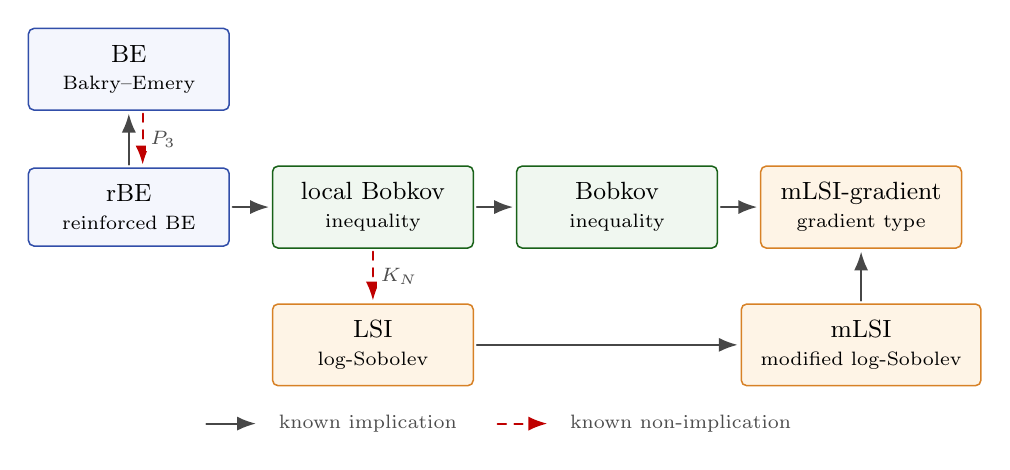
\begin{tikzpicture}[
    x=1cm,
    y=1cm,
    every node/.style={font=\small},
    box/.style={draw, rounded corners=2pt, align=center,
        inner xsep=7pt, inner ysep=6pt, minimum width=2.55cm,
        minimum height=0.86cm, line width=0.55pt},
    curvature/.style={box, draw=RoyalBlue!75!black, fill=RoyalBlue!6},
    isoperimetric/.style={box, draw=ForestGreen!70!black, fill=ForestGreen!7},
    functional/.style={box, draw=BurntOrange!85!black, fill=BurntOrange!8},
    imp/.style={-{Latex[length=2.4mm,width=1.8mm]}, draw=black!72,
        line width=0.75pt, line cap=round, shorten <=1pt, shorten >=1pt},
    noimp/.style={-{Latex[length=2.4mm,width=1.8mm]}, draw=red!75!black,
        dashed, line width=0.75pt, line cap=round,
        shorten <=1pt, shorten >=1pt},
    ann/.style={font=\scriptsize, fill=white, inner sep=1.5pt,
        text=black!70},
    legend/.style={font=\scriptsize, text=black!70}
]
    \node[curvature] (rbe) at (0,0)
        {$\mathrm{rBE}$\\[-1pt]\scriptsize reinforced BE};
    \node[isoperimetric] (localbobkov) at (3.1,0)
        {local Bobkov\\[-1pt]\scriptsize inequality};
    \node[isoperimetric] (bobkov) at (6.2,0)
        {Bobkov\\[-1pt]\scriptsize inequality};
    \node[functional] (mlsig) at (9.3,0)
        {mLSI-gradient\\[-1pt]\scriptsize gradient type};

    \node[curvature] (be) at (0,1.75)
        {$\mathrm{BE}$\\[-1pt]\scriptsize Bakry--Emery};
    \node[functional] (lsi) at (3.1,-1.75)
        {LSI\\[-1pt]\scriptsize log-Sobolev};
    \node[functional] (mlsi) at (9.3,-1.75)
        {mLSI\\[-1pt]\scriptsize modified log-Sobolev};

    \draw[imp] (rbe) -- (be);
    \draw[noimp] ([xshift=5pt]be.south) -- ([xshift=5pt]rbe.north)
        node[midway, right=1pt, ann] {$P_3$};
    \draw[imp] (rbe) -- (localbobkov);
    \draw[imp] (localbobkov) -- (bobkov);
    \draw[imp] (bobkov) -- (mlsig);
    \draw[imp] (lsi) -- (mlsi);
    \draw[imp] (mlsi) -- (mlsig);
    \draw[noimp] (localbobkov) -- (lsi)
        node[midway, right=1pt, ann] {$K_N$};

    \draw[imp] (0.95,-2.75) -- (1.65,-2.75);
    \node[legend, anchor=west] at (1.78,-2.75) {known implication};
    \draw[noimp] (4.65,-2.75) -- (5.35,-2.75);
    \node[legend, anchor=west] at (5.48,-2.75) {known non-implication};
\end{tikzpicture}
\end{center}

\begin{example}[Complete Graphs]
    Let $P(x,y) = \frac{1}{n-1}$ for all $x\neq y$.
    We have that
    $$
        Lf(x) = \frac{1}{n-1}\sum_{y\neq x}f(y) - f(x),
    $$
    $$
        \Gamma(f)(x) = \frac{1}{2(n-1)}\sum_{y\neq x}(f(y)-f(x))^2,
    $$
    $$
        L\Gamma f(x) = \frac 1{2(n-1)^2}\sum_{y\neq x}\sum_{z}(2f(z)-f(x)-f(y))(f(x)-f(y)).
    $$
    $$
        \Gamma(f,Lf)(x) = \frac{-n}{2(n-1)^2}\sum_{y\neq x}(f(y)-f(x))^2.
    $$
    Suppose $f(1) = 0$, then 
    $$
        \rho_{\-{BE}} = \min_{x,f}\frac{\Gamma_2(f)(x)}{\Gamma(f)(x)} = \min_{f}\frac{\frac{1}{4(n-1)^2}(nS-2T^2)+\frac{n}{2(n-1)^2}S}{\frac{1}{2(n-1)}S} \sim \frac 12,
    $$
    where $S = \sum_{y\neq 1}f(y)^2$ and $T = \sum_{y\neq 1}f(y)$.
    \begin{align*}
        \rho_{\-{RBE}} &= \min_{x,f}\frac{\Gamma_2(f)(x) - \Gamma(\sqrt{\Gamma(f)})(x)}{\Gamma(f)(x)} \sim \frac{\frac{1}{4(n-1)^2}(nS-2T^2)+\frac{n}{2(n-1)^2}S-\frac{n}{4(n-1)^2}S+\frac{T\sqrt{S}}{2(n-1)^2}}{\frac{1}{2(n-1)}S}\sim \frac 1{\sqrt n}.
    \end{align*}
    Since for uniform distribution
    $$
        \Ent[\mu]{f^2} \leq \frac{n\log(n-1)}{n-2}\Var[\mu]{f}
    $$
    with equality at $f = (\sqrt{n-1},1/\sqrt{n-1},\ldots,1/\sqrt{n-1})$.
    $\rho_{\-{LSI}} \sim \frac 1{\log n}$.
    For MLSI, we have that $\rho_{\-{MLSI}} \geq 1$ (LSI and MLSI are calculated by ChatGPT).
\end{example}

\section{Coordiante-wise Strong Gradient Estimate}
% \begin{figure}[htbp!]
%     \centering
%     
\includegraphics[width=0.7\textwidth]{0513_meeting_1.jpg}
%     \caption{0513 Meeting picture 1}
% \end{figure}
% \begin{figure}[htbp!]
%     \centering
%     
\includegraphics[width=0.7\textwidth]{0513_meeting_2.jpg}
%     \caption{0513 Meeting picture 2}
% \end{figure}
% \newpage
% \begin{figure}[htbp!]
%     \centering
%     
\includegraphics[width=0.7\textwidth]{0513_meeting_3.jpg}
%     \caption{0513 Meeting picture 3}
% \end{figure}
\begin{definition}
    We have the following definitions:
    weighted version of gamma calculus:
    $$
        \Gamma_wf(x) = \frac 12\sum_{i=1}^n p_i(x) w_i(x) (f(x^i)-f(x))^2 ;
    $$
    $$
        \Gamma_{w,2} f(x) = \frac 12 L \Gamma_w f - \Gamma_w(f,Lf);
    $$
    $$
        \Gamma_{w,(i)} f(x) = \frac 12 p_i(x)w_i(x)(f(x^i) - f(x))^2 .
    $$
    We say the coordinate-wise strong gradient estimate holds with constant $\rho$ if 
    $$
        \Gamma_w P_t f \leq e^{-2\rho t} \sum_{i=1}^n \tp{P_t\sqrt{\Gamma_{w,(i)} f}}^2 .
    $$
\end{definition}
\begin{theorem}[CSGE implies Talagrand's inequality (weighted version)]\label{thm:talagrand}
    Suppose the coordinate-wise strong gradient estimate holds with constant $\rho$, for any $i\in[n],x\in X$, $1/w_i(x)\leq \beta$ and log-Sobolev inequality holds with constant $\alpha$, the following is true:
    $$
        \Var[\mu]{f}\leq C(\rho,\alpha)\sum_{i=1}^n \frac{\norm{\Gamma_{w,(i)}f}_2^2}{1 + \log(\norm{\Gamma_{w,(i)}f}_2/\norm{\Gamma_{w,(i)} f}_1)}
    $$.
\end{theorem}
\begin{proof}
    We have that by reversibility,
    \begin{align*}
        -\frac 12\frac{d}{dt}\Var[\mu]{P_t f} &= \E[\mu]{\Gamma P_t f}
        \leq \beta \E[\mu]{\Gamma_w P_t f}
        \\&\leq \beta e^{-2\rho t}\E[\mu]{\sum_{i=1}^n \tp{P_t\sqrt{\Gamma_{w,(i)} f}}^2}
        \\&= \beta e^{-2\rho t}\sum_{i=1}^n \norm{P_t\sqrt{\Gamma_{w,(i)} f}}^2_{\mu,2}
        \\&\leq \beta e^{-2\rho t}\sum_{i=1}^n \norm{\sqrt{\Gamma_{w,(i)} f}}^2_{\mu,1+e^{-2\alpha t}}
        \\&\leq \beta e^{-2\rho t}\sum_{i=1}^n \norm{\sqrt{\Gamma_{w,(i)} f}}^{2\theta(t)}_{\mu,1}\norm{\sqrt{\Gamma_{w,(i)} f}}^{2-2\theta(t)}_{\mu,2} ,
        \\&= \beta e^{-2\rho t}\sum_{i=1}^n \tp{\frac{\norm{\sqrt{\Gamma_{w,(i)} f}}_{\mu,1}}{\norm{\sqrt{\Gamma_{w,(i)} f}}_{\mu,2}}}^{2\theta(t)}\norm{\sqrt{\Gamma_{w,(i)} f}}_{\mu,2}^2 .
    \end{align*}
    where $\theta(t) = \frac{1-e^{-2\alpha t}}{1+e^{-2\alpha t}}$.
    Therefore,
    $$
        \Var[\mu]{f}\leq 2\beta\sum_{i=1}^n \norm{\sqrt{\Gamma_{w,(i)} f}}_{\mu,2}^2\int_0^{\infty} e^{-2\rho t} \tp{\frac{\norm{\sqrt{\Gamma_{w,(i)} f}}_{\mu,1}}{\norm{\sqrt{\Gamma_{w,(i)} f}}_{\mu,2}}}^{2\theta(t)} dt
    $$
    Let $r_i = \frac{\norm{\sqrt{\Gamma_{w,(i)} f}}_{\mu,1}}{\norm{\sqrt{\Gamma_{w,(i)} f}}_{\mu,2}} \in [0,1]$ and $L_i = \log r_i \leq 0$.
    Since $\tanh(\alpha t)\geq \frac {\alpha t}2$ for $0\leq t\leq \frac 1\alpha$ and $\tanh(\alpha t)\geq \frac {1}2$ for $t\geq \frac 1\alpha$, we have that 
    \begin{align*}
        &\int_0^{\infty} \exp(-2\rho t + 2L_i\tanh(\alpha t)) dt
        \\&\leq\int_0^{1/\alpha} \exp(-2\rho t + L_i\alpha t) dt + \int_{1/\alpha}^{\infty} \exp(-2\rho t + L_i) dt
        \\&=\frac{1}{L_i\alpha - 2\rho}\tp{\exp\tp{L_i - \frac{2\rho}{\alpha}}-1}+\frac 1{2\rho}\exp(L_i-\frac{2\rho}{\alpha})
        \\&\leq \frac{1}{2\rho-L_i\alpha} + \frac{\exp(-2\rho/\alpha)}{2\rho}\frac{1}{1-L_i}
        \\&\leq \tp{\max\{\frac 1\alpha,\frac 1{2\rho}\}+\frac{\exp(-2\rho/\alpha)}{2\rho}}\frac{1}{1-L_i}.
    \end{align*}
    In conclusion, the following holds:
    \[
        \Var[\mu]{f}\leq C_{\beta,\alpha,\rho}\sum_{i=1}^n \frac{\norm{\Gamma_{w,(i)}f}_2^2}{1 + \log(\norm{\Gamma_{w,(i)}f}_2/\norm{\Gamma_{w,(i)} f}_1)}. \qedhere
    \]
\end{proof}
\begin{lemma}\label{lem:cBRE_condition}
    For any $i\in[n]$, $f$, the modified reinforced Bakry-\'Emery condition holds with constant $\rho$ for $\Gamma_{w,(i)}$, that is,
    $$
        \Gamma(\sqrt{\Gamma_{w,(i)}(f)}) \leq \Gamma_{w,2,(i)}(f) - \rho \Gamma_{w,(i)}(f),
    $$
    where $\Gamma_{w,2,(i)}(f) = \frac 12 L \Gamma_{w,(i)} f - \Gamma_{w,(i)}(f,Lf)$.
    Then the coordinate-wise strong gradient estimate holds with constant $\rho$.
\end{lemma}
\begin{proof}
    Define $F_s = e^{-2\rho s}\sum_{i=1}^n \tp{P_{s} \sqrt{\Gamma_{w,(i)}f_{t-s}}}^2$.
    Since $F_t = e^{-2\rho s}\sum_{i=1}^n \tp{P_{t} \sqrt{\Gamma_{w,(i)}f}}^2$, $F_0 = \Gamma_w f_t$, if $F_s$ is monotone increasing, that is, $\frac d{ds}F_s \geq 0$, then we finish the proof.
    Let $g_{i,s} = P_s\sqrt{\Gamma_{w,(i)}f_{t-s}}$, $h_{i,s} = \sqrt{\Gamma_{w,(i)}f_{t-s}}$.
    We have that
    \begin{align}
        \frac d{ds} F_s &= e^{-2\rho s}\Bigg(-2\rho \sum_{i=1}^n g_{i,s}^2 + 2\sum_{i=1}^n g_{i,s}\left(Lg_{i,s} + P_s\left(\frac{-2\Gamma_{w,i}(f_{t-s},Lf_{t-s})}{2h_{i,s}}\right)\right)\Bigg) \nonumber
        \\&=2e^{-2\rho s}\sum_{i=1}^n g_{i,s}\Bigg(-\rho g_{i,s} + Lg_{i,s} + P_s\left(\frac{-\Gamma_{w,i}(f_{t-s},Lf_{t-s})}{h_{i,s}}\right)\Bigg) \nonumber
        \\&= 2e^{-2\rho s}\sum_{i=1}^n g_{i,s}P_s\Bigg(-\rho \sqrt{\Gamma_{w,(i)}f_{t-s}} + L\sqrt{\Gamma_{w,(i)}f_{t-s}} - \frac{\Gamma_{w,i}(f_{t-s},Lf_{t-s})}{h_{i,s}}\Bigg). \label{eq:NTS}
    \end{align}
    Now it is sufficient to show that
    \begin{align*}
        -\rho h_{i,s} + Lh_{i,s} - \frac{\Gamma_{w,i}(f_{t-s},Lf_{t-s})}{h_{i,s}} &\geq 0
       \\\iff h_{i,s}Lh_{i,s} - \Gamma_{w,i}(f_{t-s},Lf_{t-s}) &\geq \rho \Gamma_{w,(i)}f_{t-s}
       \\\iff \frac 12L(\Gamma_{w,(i)}f_{t-s})-\Gamma(h_{i,s})+\Gamma_{w,2,(i)}f_{t-s} - \frac 12L(\Gamma_{w,(i)}f_{t-s}) &\geq \rho \Gamma_{w,(i)}f_{t-s}
       \\\iff \Gamma_{w,2,(i)}f_{t-s} - \rho \Gamma_{w,(i)}f_{t-s} &\geq \Gamma(\sqrt{\Gamma_{w,(i)}f_{t-s}}). \qedhere
    \end{align*}
\end{proof}
\begin{remark}
    Usually Lemma \ref{lem:cBRE_condition} is too strong to check.
    We should check Equation \ref{eq:NTS} instead.
\end{remark}
Let us consider the zero-field Ising model and the following transition matrix,
$$
    \forall x\in \{\pm 1\}^n, \mu(x) \propto \exp(\frac12 x^\top J x) , P(x,x^i) \propto \sqrt{\mu(x^i)/\mu(x)} .
$$
Trivially the reversibility holds.
\begin{example}[CSGE fails when $w = 1$]
    Suppose $J_{ij} \neq 0$ and fix $x$ with $\-{sign}(x_ix_j) = \-{sign}(J_{ij})$.
    Let 
    $$
        f(y) = \begin{cases}\eps, &y=x^i\\1, &y=x^{ij}\\ 0, &\text{o.w.}\end{cases} .
    $$
    Let $H(t) = e^{-2\rho t}\norm{P_t\sqrt{\Gamma_{(k)}(f)(x)}}_2^2 - \Gamma f_t(x)$.
    Since $H(0) = 0$, it is sufficient to show that $H'(t) < 0$.
    We have that 
    \begin{align*}
        H'(t) = 2e^{-2\rho t}\tp{-\rho\norm{P_t\sqrt{\Gamma_{(k)}(f)}(x)}_2^2 + \sum_{k=1}^n P_t \sqrt{\Gamma_{(k)} f}(x)P_t L \sqrt{\Gamma_{(k)} f}(x)}- 2\Gamma(f_t,Lf_t)(x)
    \end{align*}
    Since 
    $$
        2\Gamma(f,Lf)(x) = \eps p_i(x)(Lf(x^i) - Lf(x)) = \eps p_i(x)\bigg((1-p_i(x))\eps - p_j(x^i)\bigg);
    $$
    $$
        \norm{\sqrt{\Gamma_{(k)}(f)}(x)}_2^2 = \frac 12p_i(x)\eps^2; \quad \sqrt{\Gamma_{(i)} f}(x)L \sqrt{\Gamma_{(i)} f}(x) = O(\eps^2) + \sqrt{p_i(x)p_i(x^j)}p_j(x)\eps
    $$
    Therefore,
    $$
        H'(0) = O_\rho(\eps^2)+p_j(x)\sqrt{p_i(x^j)}\tp{\sqrt{p_i(x)}-\sqrt{p_i(x^j)}}\eps .
    $$
    Since $p_i(x^j) = p_i(x)\exp(2x_ix_jJ_{ij})$, $\sqrt{p_i(x)}-\sqrt{p_i(x^j)} < 0$.
    Let $\eps$ tend to $0^+$, $H'(0) < 0$.

\end{example}
For $J = 0$ and $w = 1$, $\rho_{CSGE} = 2$ which is calculated by ChatGPT.

\begin{lemma}[CSGE for when $w = p$]\label{lem:CSGE_w=p}
    Let $w=p$.
    Suppose $P(x,x^i)P(x^i,x^{ij})=P(x,x^j)P(x^j,x^{ij})$ and $P(x,x^i)P(x^i,x)=1$.
    Define $H_{ij} = \frac{p_i(x^j)}{p_i(x)} = \frac{p_j(x^i)}{p_j(x)}$.
    Then the coordinate-wise strong gradient estimate holds with constant $\rho \leq \lambda_{\min}(\diag\{2\alpha-\beta\*1\} - \frac{\beta+\beta^{\top}}{2})$, where
    $$
        \forall i,\alpha_i = \min_x \frac{1}{p_i(x)}\quad \text{and}\quad\forall i\neq j, \beta_{ij} = \max_x|1-H_{ij}(x)|p_j(x), \beta_{ii}=0.
    $$
\end{lemma}
\begin{proof}
    Define $d_i = f(x^i) - f(x)$, $d_{ij} = f(x^{ij})-f(x^i)-f(x^j)+f(x)$ and $H_{ij} = \frac{p_i(x^j)}{p_i(x)} = \frac{p_j(x^i)}{p_j(x)}$.% = e^{2J_{ij}x_ix_j}$.
    We omit $(x)$ for simplicity if it is clear.
    We have that 
    $$
        \Gamma_{w,(i)}(f,Lf) = \frac 12p_i^2d_i\sum_{j\in [n]}p_j(x^i)(d_{ij}+d_j)-p_jd_j
        = \frac 12 p_i^2d_i\tp{-(\frac{1}{p_i}+p_i)d_i+\sum_{j\neq i}H_{ij}p_j(d_{ij}+d_j)-p_jd_j}
    $$
    Define $A_{\rho,i} = -\rho \sqrt{\Gamma_{w,(i)}f_{}} + L\sqrt{\Gamma_{w,(i)}f_{}} - \frac{\Gamma_{w,i}(f_{},Lf_{})}{\sqrt{\Gamma_{w,(i)}f}}$.
    We have that
    \begin{align}
        A_{\rho,i}& = -\frac{\rho}{\sqrt{2}}p_i\abs{d_i} + \frac{(1+p_i^2)\sgn(d_i)d_i+(1-p_i^2)|d_i|}{\sqrt{2}} \nonumber
        \\&+\sum_{j\neq i}\frac{p_ip_j}{\sqrt 2}(H_{ij}\abs{d_{ij}+d_i}-\abs{d_i} + \sgn(d_i)d_j-\sgn(d_i)H_{ij}(d_{ij}+d_j)) \nonumber
        \\&=\frac{2-\rho p_i}{\sqrt 2}|d_i|+\sum_{j\neq i}\frac{p_ip_j}{\sqrt 2}\bigg(H_{ij}\abs{d_{ij}+d_i}-\sgn(d_i)H_{ij}(d_{ij}+d_j)+\sgn(d_i)(d_j-d_i)\bigg) \nonumber
        \\&\geq \frac{2-\rho p_i}{\sqrt 2}|d_i|+\sum_{j\neq i}\frac{p_ip_j}{\sqrt 2}\sgn(d_i)(1-H_{ij})(d_j-d_i) \nonumber
        \\&\geq \frac{2-\rho p_i}{\sqrt 2}|d_i|-\sum_{j\neq i}\frac{p_ip_j}{\sqrt 2}|1-H_{ij}|(|d_j|+|d_i|) ,\label{eq:A_rhoi_lower_bound}
    \end{align}
    since $|a|+\sgn(\cdot)a\geq 0$.
    Therefore, for any $s\geq 0$, let $v_i = p_i|d_i|$, we have that 
    \begin{align*}
        \sum_{i=1}^n P_s \frac{p_i}{\sqrt 2}|d_i|P_s A_{\rho,i}
        &\geq \frac 12\sum_{i=1}^n P_sv_iP_s\bigg((\frac{2}{p_i}-\rho - \sum_{j\neq i}\abs{1-H_{ij}}p_j)v_i - \sum_{j\neq i}\abs{1-H_{ij}}p_iv_j\bigg)
        \\&\geq \frac 12\sum_{i=1}^n P_sv_iP_s\bigg((2\alpha_i-\rho - \sum_{j\neq i}\beta_{ij})v_i - \sum_{j\neq i}\beta_{ji}v_j\bigg)
        \\&=(P_sv)^\top \bigg(\diag\{2\alpha-\beta\*1\}-\rho I- \frac{\beta+\beta^{\top}}{2}\bigg) (P_sv)
    \end{align*}
    where $\alpha_i = \min_x \frac{1}{p_i(x)}$, $\beta_{ij} = \max_x|1-H_{ij}(x)|p_j(x)$ for $i\neq j$ and $\beta_{ii}=0$.
    By Equation \ref{eq:NTS}, the coordinate-wise strong gradient estimate holds with constant $\rho$ if $\diag\{2\alpha-\beta\*1\}-\rho I- \frac{\beta+\beta^{\top}}{2}\succeq 0$, that is,
    $\rho \leq \lambda_{\min}(\diag\{2\alpha-\beta\*1\} - \frac{\beta+\beta^{\top}}{2})$.
\end{proof}
\begin{corollary}[Zero field Ising model]
    For $\mu(x) \propto \exp(\frac 12 x^\top J x)$ with $J_{ii}=0$, $J^\top = J$ and $\norm{J}_1= B$, where $2e^{-2B}-4Be^{2B} \geq 0$.
    If $P_i(x) = \sqrt{\mu(x^i)/\mu(x)}$, then $\rho_{CSGE} = 2e^{-2B}-4Be^{2B}$.
\end{corollary}
\begin{proof}
    We have that $p_i(x) = \exp(-2x_ix^\top J_i)\in [e^{-2B},e^{2B}]$ and
    $$
       \beta_{ij} = \max_x \abs{\exp(-2x_jx^\top J_j)-\exp\tp{2x_j(-x^\top J_j+x_iJ_{i,j})}} \leq (1-e^{-2|J_{i,j}|})e^{2B} \leq 2|J_{i,j}|e^{2B}.
    $$
    By Gershgorin circle theorem, we have that
    \[
        \lambda_{\min}(\diag\{2\alpha-\beta\*1\} - \frac{\beta+\beta^{\top}}{2})
        \geq 2e^{-2B} - \frac {\norm{\beta}_1+3\norm{\beta}_\infty}2 \geq 2e^{-2B}-4Be^{2B} . \qedhere
    \]
\end{proof}

\begin{lemma}[CSGE for non-symmetric version]
    Define $H_{ij} = \frac{p_i(x^j)}{p_i(x)}$ and $W_{ij} = \frac{w_i(x^j)}{w_i(x)}$.
    If $\sqrt{H_{ij}W_{ij}} \geq H_{ji}$,
    then coordinate-wise strong gradient estimate holds with constant $\rho \leq \lambda_{\min}(\diag\{\alpha\} - \frac{\beta+\beta^{\top}}{2})$, 
    where 
    $$
        \alpha_i = \min_x p_i\sqrt{H_{ii}W_{ii}} + p_iH_{ii} - \sum_{j\neq i}p_j\abs{1-H_{ji}},
    $$
    $$
        \beta_{ij} = p_j|1-H_{ji}|\sqrt{\frac{p_iw_i}{p_jw_j}}\text{ for $i\neq j$ and $\beta_{ii}=0$ }.
    $$
\end{lemma}
\begin{proof}
    Define $d_i = f(x^i) - f(x)$, $d_{ij} = f(x^{ij})-f(x^i)-f(x^j)+f(x)$, $H_{ij} = \frac{p_i(x^j)}{p_i(x)}$ and $W_{ij} = \frac{w_i(x^j)}{w_i(x)}$.
    We omit $(x)$ for simplicity if it is clear.
    We have that 
    $$
        \Gamma_{w,(i)}(f,Lf) = \frac 12p_iw_id_i\sum_{j\in [n]}p_j(x^i)(d_{ij}+d_j)-p_jd_j
        = \frac 12 p_iw_id_i\tp{-(H_{ii}p_i+p_i)d_i+\sum_{j\neq i}H_{ji}p_j(d_{ij}+d_j)-p_jd_j}.
    $$
    Define $A_{\rho,i} = -\rho \sqrt{\Gamma_{w,(i)}f_{}} + L\sqrt{\Gamma_{w,(i)}f_{}} - \frac{\Gamma_{w,i}(f_{},Lf_{})}{\sqrt{\Gamma_{w,(i)}f}}$.
    We have that
    \begin{align}
        A_{\rho,i}& = \sqrt{\frac {p_iw_i}2}|d_i|(p_i\sqrt{H_{ii}W_{ii}} + p_iH_{ii}-\rho) \nonumber
        \\&+\sqrt{\frac {p_iw_i}2}\sum_{j\neq i}p_j(\sqrt{H_{ij}W_{ij}}|d_i+d_{ij}|-|d_i|-\sgn(d_i)H_{ji}(d_j+d_{ij}+d_i-d_i)+\sgn(d_i)d_j) \nonumber
        \\&\geq \sqrt{\frac {p_iw_i}2}|d_i|(p_i\sqrt{H_{ii}W_{ii}} + p_iH_{ii}-\rho) + \sqrt{\frac {p_iw_i}2}\sum_{j\neq i}p_j(1-H_{ji})\sgn(d_i)(d_j-d_i) \label{eq:CSGE_nonsym_Check}
        \\&\geq \sqrt{\frac {p_iw_i}2}|d_i|(p_i\sqrt{H_{ii}W_{ii}} + p_iH_{ii}-\rho) - \sqrt{\frac {p_iw_i}2}\sum_{j\neq i}p_j|1-H_{ji}|(|d_j|+|d_i|), \nonumber
    \end{align}
    where Equation \ref{eq:CSGE_nonsym_Check} holds if 
    $$
        \sqrt{H_{ij}W_{ij}} \geq H_{ji} \iff \sqrt{\frac{p_i(x^j)w_i(x^j)}{p_i(x)w_i(x)}}\geq \frac{p_j(x^i)}{p_j(x)} .
    $$
    Therefore, for any $s\geq 0$, let $v_i = \sqrt{w_ip_i}|d_i|$, we have that 
    \begin{align*}
        \sum_{i=1}^n P_s \frac{\sqrt{p_iw_i}}{\sqrt 2}|d_i|P_s A_{\rho,i}
        &\geq \frac 12\sum_{i=1}^n P_sv_iP_s\bigg(v_i(p_i\sqrt{H_{ii}W_{ii}} + p_iH_{ii}-\rho - \sum_{j\neq i}p_j\abs{1-H_{ji}}) - \sum_{j\neq i}p_j|1-H_{ji}|\sqrt{\frac{p_iw_i}{p_jw_j}}v_j\bigg)
        \\&= \frac 12(P_sv)^\top \bigg(\diag\{\alpha\}-\rho I- \frac{\beta+\beta^{\top}}{2}\bigg) (P_sv) .
    \end{align*}
    By Equation \ref{eq:NTS}, the coordinate-wise strong gradient estimate holds with constant $\rho$ if $\diag\{\alpha\}-\rho I- \frac{\beta+\beta^{\top}}{2}\succeq 0$, that is,
    $\rho \leq \lambda_{\min}(\diag\{\alpha\} - \frac{\beta+\beta^{\top}}{2})$.
\end{proof}
\section{Decay of 2-norm of influnces}
We have the following definitions:
$$
    I_i(f_{t-s}) := \frac 1{\sqrt 2}\norm{\delta_i f}_{1,i} = \frac 1{\sqrt 2}\E[\mu]{p_i\abs{\delta_i f}} = \E[\mu]{\sqrt{\Gamma_{p,(i)}f}},
$$
$$
    W(f) := \sum_{i=1}^n I_i(f_{t-s})^2 = \sum_{i=1}^n \E[\mu]{\sqrt{\Gamma_{p,(i)}f}}^2 .
$$
We say $W$-decay holds if for any function $f: \{\pm 1\}^n \mapsto \R$, $W(P_t f)\leq e^{-2\rho t}W(f)$. 
% In the following calculation, we ignore $\sqrt{2}$ in influences for simplicity.
\begin{lemma} 
    Suppose $P(x,x^i)P(x^i,x^{ij})=P(x,x^j)P(x^j,x^{ij})$ and $P(x,x^i)P(x^i,x)=1$.
    Define $H_{ij} = \frac{p_i(x^j)}{p_i(x)} = \frac{p_j(x^i)}{p_j(x)}$.
    Then the $W$-decay holds with constant $\rho \leq \lambda_{\min}(\diag\{2\alpha-\beta\*1\} - \frac{\beta+\beta^{\top}}{2})$, where
    $$
        \forall i,\alpha_i = \min_x \frac{1}{p_i(x)}\quad \text{and}\quad\forall i\neq j, \beta_{ij} = \max_x|1-H_{ij}(x)|p_j(x), \beta_{ii}=0.
    $$
\end{lemma}
\begin{proof}
    Define 
    $$
        F_s = e^{-2\rho s}\sum_{i=1}^n\E[\mu]{P_s\sqrt{\Gamma_{p,i}(f_{t-s})}}^2 = e^{-2\rho s}W(f_{t-s}).
    $$
    Note that $F_0 = W(f_t)$ and $F_t = e^{-2\rho t}W(f)$.
    We have that
    \begin{align*}
        \frac{d}{ds} F_s &= e^{-2\rho s}\tp{-2\rho W(f_{t-s}) + 2\sum_{i=1}^n I_i(f_{t-s})\E[\mu]{P_sL\sqrt{\Gamma_{p,i}(f_{t-s})}+P_s\tp{\frac{-\Gamma_{p,i}(f_{t-s},Lf_{t-s})}{\sqrt{\Gamma_{p,i} f_{t-s}}}}}}
        \\&= e^{-2\rho s}\sum_{i=1}^nI_i(f_{t-s})\tp{\E[\mu]{P_s\tp{-2\rho \sqrt{\Gamma_{p,i}f_{t-s}} + 2L\sqrt{\Gamma_{p,i}(f_{t-s})}-\frac{2\Gamma_{p,i}(f_{t-s},Lf_{t-s})}{\sqrt{\Gamma_{p,i} f_{t-s}}}}}} .
    \end{align*}
    By Equation \ref{eq:A_rhoi_lower_bound}, we have that
    \begin{align*}
        &\E[\mu]{P_s\tp{-\rho \sqrt{\Gamma_{p,i}f_{t-s}} + L\sqrt{\Gamma_{p,i}(f_{t-s})}-\frac{\Gamma_{p,i}(f_{t-s},Lf_{t-s})}{\sqrt{\Gamma_{p,i} f_{t-s}}}}}
        \\\geq& \frac 1{\sqrt 2}\E[\mu]{\tp{\frac{2}{p_i} - \rho - \sum_{j\neq i}\abs{1-H_{ij}}p_j}p_i|d_i| - p_i\sum_{j\neq i}p_j|1-H_{ij}||d_j|}
        \\\geq& \frac 1{\sqrt 2}\tp{(2\alpha - \rho - \sum_{j\neq i}\beta_{ij})I_i(f_{t-s}) - \sum_{j\neq i}\beta_{ji}I_j(f_{t-s})}.
    \end{align*}
    Following the same calculation in Lemma \ref{lem:CSGE_w=p}, $\frac{d}{ds} F_s \geq 0$ if $\rho \leq \lambda_{\min}(\diag\{2\alpha - \beta\*1\} - \frac {\beta + \beta^\top}2)$ .
    % Therefore, it is sufficient to check
    % $$
    %     -\rho \sqrt{\Gamma_{p,i}f_{t-s}} + 2L\sqrt{\Gamma_{p,i}(f_{t-s})}-\frac{2\Gamma_{p,i}(f_{t-s},Lf_{t-s})}{\sqrt{\Gamma_{p,i} f_{t-s}}} \geq 0
    % $$
    % $$
    %     \iff 2\Gamma_{p,2,i} (f_{t-s}) - \rho \Gamma_{p,i}(f_{t-s}) \geq 2\Gamma(\sqrt{\Gamma_{w,i}(f_{t-s})}) .
    % $$
    % Or check
    % $$
    %     \sum_{i=1}^n I_i(f_{t-s})\E[\mu]{-\rho \sqrt{\Gamma_{p,i}(f_{t-s})} + 2L\sqrt{\Gamma_{p,i}(f_{t-s})}-\frac{2\Gamma_{p,i}(f_{t-s},Lf_{t-s})}{\sqrt{\Gamma_{p,i} f_{t-s}}}} \geq 0
    % $$
\end{proof}
Define
$$
    \+B(f) = \sum_{i=1}^n \norm{\sqrt{\Gamma_{w,(i)}f}}_2^2 = \E[\mu]{\Gamma_wf}, \+A(f) = \sum_{i=1}^n \norm{\sqrt{\Gamma_{w,(i)}f}}_1^2.
$$
Note that $\+A(f) = W(f)$ if $w = p$.
\begin{proposition}[]\label{prop:Tala_upper}
    $$
        \sum_{i=1}^n \frac{\norm{\sqrt{\Gamma_{w,(i)}f}}_2^2}{1 + \log(\norm{\sqrt{\Gamma_{w,(i)}f}}_2/\norm{\sqrt{\Gamma_{w,(i)}f}}_1)}
        \lesssim \frac{\+B(f)}{1 + \log(\sqrt{\+B(f)/\+A(f)})}
    $$
\end{proposition}
\begin{proof}
Define $I = \{i\in [n]\mid \norm{\sqrt{\Gamma_{w,(i)}f}}_2/\norm{\sqrt{\Gamma_{w,(i)}f}}_1 \geq (\+B(f)/\+A(f))^{1/4}\}$.
Then we have that
\begin{equation}\label{eq:Tala_upper_1}
    \sum_{i\in I} \frac{\norm{\sqrt{\Gamma_{w,(i)}f}}_2^2}{1 + \log(\norm{\sqrt{\Gamma_{w,(i)}f}}_2/\norm{\sqrt{\Gamma_{w,(i)}f}}_1)}
    \leq \sum_{i\in [n]} \frac{2\norm{\sqrt{\Gamma_{w,(i)}f}}_2^2}{1 + \log(\sqrt{\+B(f)/\+A(f)})} 
    = 2\frac{\+B(f)}{1 + \log(\+B(f)/\+A(f))}
\end{equation}
Since $\norm{\sqrt{\Gamma_{w,(i)}f}}_2 \geq \norm{\sqrt{\Gamma_{w,(i)}f}}_1$, 
\begin{align}
    \sum_{i\notin I} \frac{\norm{\sqrt{\Gamma_{w,(i)}f}}_2^2}{1 + \log(\norm{\sqrt{\Gamma_{w,(i)}f}}_2/\norm{\sqrt{\Gamma_{w,(i)}f}}_1)}
    &\leq \sqrt{\frac{\+B(f)}{\+A(f)}}\sum_{i\notin I}\norm{\sqrt{\Gamma_{w,(i)}f}}_1^2 \nonumber
    \\&= \sqrt{\frac{\+A(f)}{\+B(f)}}\+B(f)
    \leq \frac{\+B(f)}{1 + \log(\+B(f)/\+A(f))} \label{eq:Tala_upper_2}.
\end{align}
Combining Equation \ref{eq:Tala_upper_1} and \ref{eq:Tala_upper_2}, we conclude the proof.
\end{proof}
\begin{lemma}[Smoothing lemma]
    Suppose $\mu$ is fully supported. 
    Under the Talagrand inequality assumption with constant $C_{\rho,\alpha,\beta}$ and $W$-decay holds with constant $\rho$.
    We have that for any $t\geq 0$,
    $$
        \Var[\mu]{P_t f} \leq 3C_{\rho,\alpha,\beta}\cdot \Var[\mu]{f}^{\theta(t)}W(f)^{1-\theta(t)},
    $$
    where $\theta(t) = e^{-2t/3C_{\rho,\alpha,\beta}\beta}$.
\end{lemma}
\begin{proof}
    We may assume $W(f)\neq 0$, $\Var[\mu]{f} \neq 0$ and $W(f) \leq \Var[\mu]{f}$.
    Let $w = p$.
    By Theorem \ref{thm:talagrand} and Proposition \ref{prop:Tala_upper}, we conclude that
    $$
        \frac{\Var[\mu]{f}}{C_{\rho,\alpha,\beta}\+A(f)}\leq 3\frac{\+B(f)/\+A(f)}{1+\log(\+B(f)/\+A(f))} \implies \+B(f)\geq \frac{\Var[\mu]{f}}{3C_{\rho,\alpha,\beta}}(1 + \log \frac{\Var[\mu]{f}}{3C_{\rho,\alpha,\beta}\+A(f)}),
    $$
    since $y\leq \frac{x}{1+\log x}$ implies $x\geq y(1+\log y)$ for $x\geq 1$.
    By $W$-decay,
    \begin{align*}
        -\frac{d}{dt}\Var[\mu]{f_t} = 2\E[\mu]{\Gamma P_t f} \geq \frac 2{\beta} \E[\mu]{\Gamma_p f_t}
        &\geq \frac 2{\beta} \frac{\Var[\mu]{f_t}}{3C_{\rho,\alpha,\beta}}\tp{1 + \log \frac{\Var[\mu]{f_t}}{3C_{\rho,\alpha,\beta}\+A(f_t)}}
        \\&\geq \frac 2{\beta} \frac{\Var[\mu]{f_t}}{3C_{\rho,\alpha,\beta}}\tp{1 + \log \frac{\Var[\mu]{f_t}}{3C_{\rho,\alpha,\beta}W(f)}} .
    \end{align*}
    Let $z(t) = 1 + \log \frac{\Var[\mu]{f_t}}{CW(f)}$ and $C = 3C_{\rho,\alpha,\beta}$, the above inequality is equivalent to 
    $$
        z'(t) \leq \frac{-2}{C\beta}z(t) \implies \Var[\mu]{f_t}\leq CW(f)\exp\tp{e^{-2t/C\beta}\tp{1+\log \frac{\Var[\mu]{f}}{CW(f)}} - 1}.
    $$
    In conclusion, we have that
    $$
        \Var[\mu]{f_t} \leq C^{1-\theta(t)}e^{\theta(t)-1}\Var[\mu]{f}^{\theta(t)}W(f)^{1-\theta(t)},
    $$
    where $\theta(t) = e^{-2t/C\beta}$.
\end{proof}
\end{document}
